\documentclass{article}
\usepackage[utf8]{inputenc}
\usepackage{listings}

\lstset{
    basicstyle=\ttfamily\footnotesize,
    breaklines=true,
    columns=fullflexible,
    frame=single,
    captionpos=b
}

\title{Final Assignment: Computer Workshop Course}
\author{Hazhir Yousefi}
\date{\today}

\begin{document}

\maketitle

\tableofcontents

\section{Git and GitHub}
\subsection{Repository Initialization and Commits}
To start this assignment, I created a new repository on GitHub named `latex`. Below are the steps I followed:

\begin{enumerate}
    \item Created the repository on GitHub and added a `.gitignore` file for LaTeX to avoid unnecessary files being tracked.
    \item Cloned the repository to my local machine using the command:
    \begin{verbatim}
    git clone https://github.com/Hazhir2002/latex
    cd latex
    \end{verbatim}
    \item Created a basic LaTeX document named `assignment.tex` and structured it with sections for each task.
    \item Made meaningful commits regularly as I progressed. For instance:
    \begin{verbatim}
    git add assignment.tex
    git commit -m "Add initial structure of LaTeX document"
    git push
    \end{verbatim}
\end{enumerate}

\subsection{GitHub Actions for LaTeX Compilation}
To automate the compilation of my LaTeX document, I set up a GitHub Actions workflow. Below are the steps I followed:

\begin{enumerate}
    \item Created a new directory in my repository named `.github/workflows` and added a file named `latex.yml`.
    \item Wrote the following workflow code:
    \begin{verbatim}
      name: Build and Release LaTeX Document

      on:
        push:
          tags:
            - "*"
      
      permissions:
        contents: write
      
      jobs:
        build:
          runs-on: ubuntu-latest
          steps:
            - name: Checkout Repository
              uses: actions/checkout@v3
      
            - name: Set up LaTeX
              run: sudo apt-get update && sudo apt-get install -y texlive-full
      
            - name: Compile LaTeX Document
              run: pdflatex -interaction=nonstopmode -halt-on-error 
              -file-line-error assignment.tex
      
            - name: Create Release
              id: create_release
              uses: actions/create-release@v1
              env:
                GITHUB_TOKEN: ${{ secrets.GITHUB_TOKEN }}
              with:
                tag_name: ${{ github.ref_name }}
                release_name: Release ${{ github.ref_name }}
                draft: false
                prerelease: false
      
            - name: Upload Compiled PDF
              uses: actions/upload-release-asset@v1
              env:
                GITHUB_TOKEN: ${{ secrets.GITHUB_TOKEN }}
              with:
                upload_url: ${{ steps.create_release.outputs.upload_url }}
                asset_path: ./assignment.pdf
                asset_name: assignment.pdf
                asset_content_type: application/pdf
    \end{verbatim}
    \item Committed the workflow file and pushed it to GitHub.
    \item Created a tag using the following commands to test the workflow:
    \begin{verbatim}
    git tag v1.0
    git push origin v1.0
    \end{verbatim}
    \item Verified that the workflow successfully compiled the LaTeX document and uploaded the PDF to the "Releases" section of the repository.
\end{enumerate}

\section{Exploration Tasks}
\subsection{Vim Advanced Features}
\subsubsection{Macros}
Macros allow you to record and replay sequences of commands, which is useful for repetitive tasks.
\begin{enumerate}
    \item Press \texttt{q} followed by a register name (e.g., \texttt{q a} to record in register \texttt{a}).
    \item Perform the actions you want to record.
    \item Press \texttt{q} again to stop recording.
    \item Replay the macro with \texttt{@a}.
    \item Repeat multiple times using \texttt{N@a} (replace \texttt{N} with a number).
\end{enumerate}

\subsubsection{Visual Block Mode}
Visual Block Mode allows you to select and manipulate text in a rectangular block.
\begin{enumerate}
    \item Press \texttt{Ctrl + v} to enter visual block mode.
    \item Use arrow keys to select a rectangular area.
    \item Press \texttt{I} (insert) or \texttt{A} (append) to modify the block.
    \item Hit \texttt{Esc} to apply the changes.
\end{enumerate}

\subsubsection{Splits and Buffers}
Splits and Buffers allow you to work with multiple files or views simultaneously.
\begin{enumerate}
    \item Open a horizontal split with \texttt{:split} or a vertical split with \texttt{:vsplit}.
    \item Navigate between splits with \texttt{Ctrl + w} and arrow keys.
    \item List open buffers with \texttt{:ls} and switch with \texttt{:b<N>} (replace \texttt{<N>} with the buffer number).
\end{enumerate}

\subsection{Memory Profiling}

\subsubsection{Memory Leak}
A memory leak occurs when a program allocates memory dynamically but fails to release it after use. Over time, this can cause the system to run out of memory, leading to crashes or poor performance.
\begin{lstlisting}[language=C]
int *ptr = malloc(sizeof(int) * 100);
// Forget to free the memory: free(ptr);
\end{lstlisting}

\subsubsection{Memory Profilers}
\textbf{Purpose of Valgrind:}
Valgrind is a tool that helps detect memory-related issues such as leaks, invalid accesses, and uninitialized memory.
\begin{itemize}
    \item Identifies locations of memory leaks in your code.
    \item Tracks memory usage and helps optimize memory allocation.
\end{itemize}
\textbf{Example Command:}
\begin{lstlisting}[language=bash]
valgrind --leak-check=full ./your_program
\end{lstlisting}

\subsection{GNU/Linux Bash Scripting}

\subsubsection{fzf}
\textbf{What is Fuzzy Searching?}
Fuzzy searching matches approximate strings instead of exact matches. It’s useful when you don’t remember the exact name or details of what you’re looking for.

\textbf{Command Explanation:}
\begin{lstlisting}[language=bash]
ls | fzf
\end{lstlisting}
This lists all files and directories (\texttt{ls}) and pipes them to \texttt{fzf}, which allows you to interactively search and filter the results.

\subsubsection{Using fzf to Find Your Favorite PDF}
\begin{enumerate}
  \item \textbf{Command to List All PDFs:}
  \begin{lstlisting}[language=bash]
  fd . --extension pdf
  \end{lstlisting}

  \item \textbf{Command to Use fzf for Selection:}
  \begin{lstlisting}[language=bash]
  fd . --extension pdf | fzf
  \end{lstlisting}
\end{enumerate}

\subsubsection{Opening the File Using Zathura}
\textbf{Command to Open PDF:}
\begin{lstlisting}[language=bash]
zathura $(fd . --extension pdf | fzf)
\end{lstlisting}
This command combines \texttt{fd}, \texttt{fzf}, and \texttt{zathura}:
\begin{enumerate}
    \item \texttt{fd} lists all PDFs.
    \item \texttt{fzf} lets you interactively select one.
    \item \texttt{zathura} opens the selected file.
\end{enumerate}

\newpage

\section{Git and FOSS}
\subsection{README.md}
The \texttt{README.md} file is an essential component of any GitHub repository, as it provides a quick overview of the repository's purpose and contents. For this assignment, the \texttt{README.md} includes:
\begin{itemize}
    \item The title of the repository.
    \item A brief description of the repository's aim.
    \item A list of the key features and components.
    \item Instructions for compiling the \LaTeX{} document and contributing to the repository.
\end{itemize}

Here is the content of the \texttt{README.md} file:
\begin{lstlisting}[language=markdown]
# Final Assignment Repository

This repository contains the final assignment for the Computer Workshop course. It demonstrates skills in Git, \LaTeX{}, GitHub Actions, and more.

## Features
- A structured \LaTeX{} document answering all assignment questions.
- Automated compilation of the \LaTeX{} document into a PDF using GitHub Actions.
- A demonstration of Git and FOSS practices.

## Usage
1. Clone the repository.
2. Edit the \LaTeX{} document (\texttt{assignment.tex}).
3. Commit and push changes to trigger GitHub Actions and generate a new release.
4. Download the compiled PDF from the \texttt{Releases} section.
\end{lstlisting}

\subsection{Issues}
As part of this assignment, a sample issue was created in the repository located at \url{https://github.com/MiliAxe/CW-Final}. Below is a screenshot of the created issue:

\begin{figure}[h!]
 \centering
 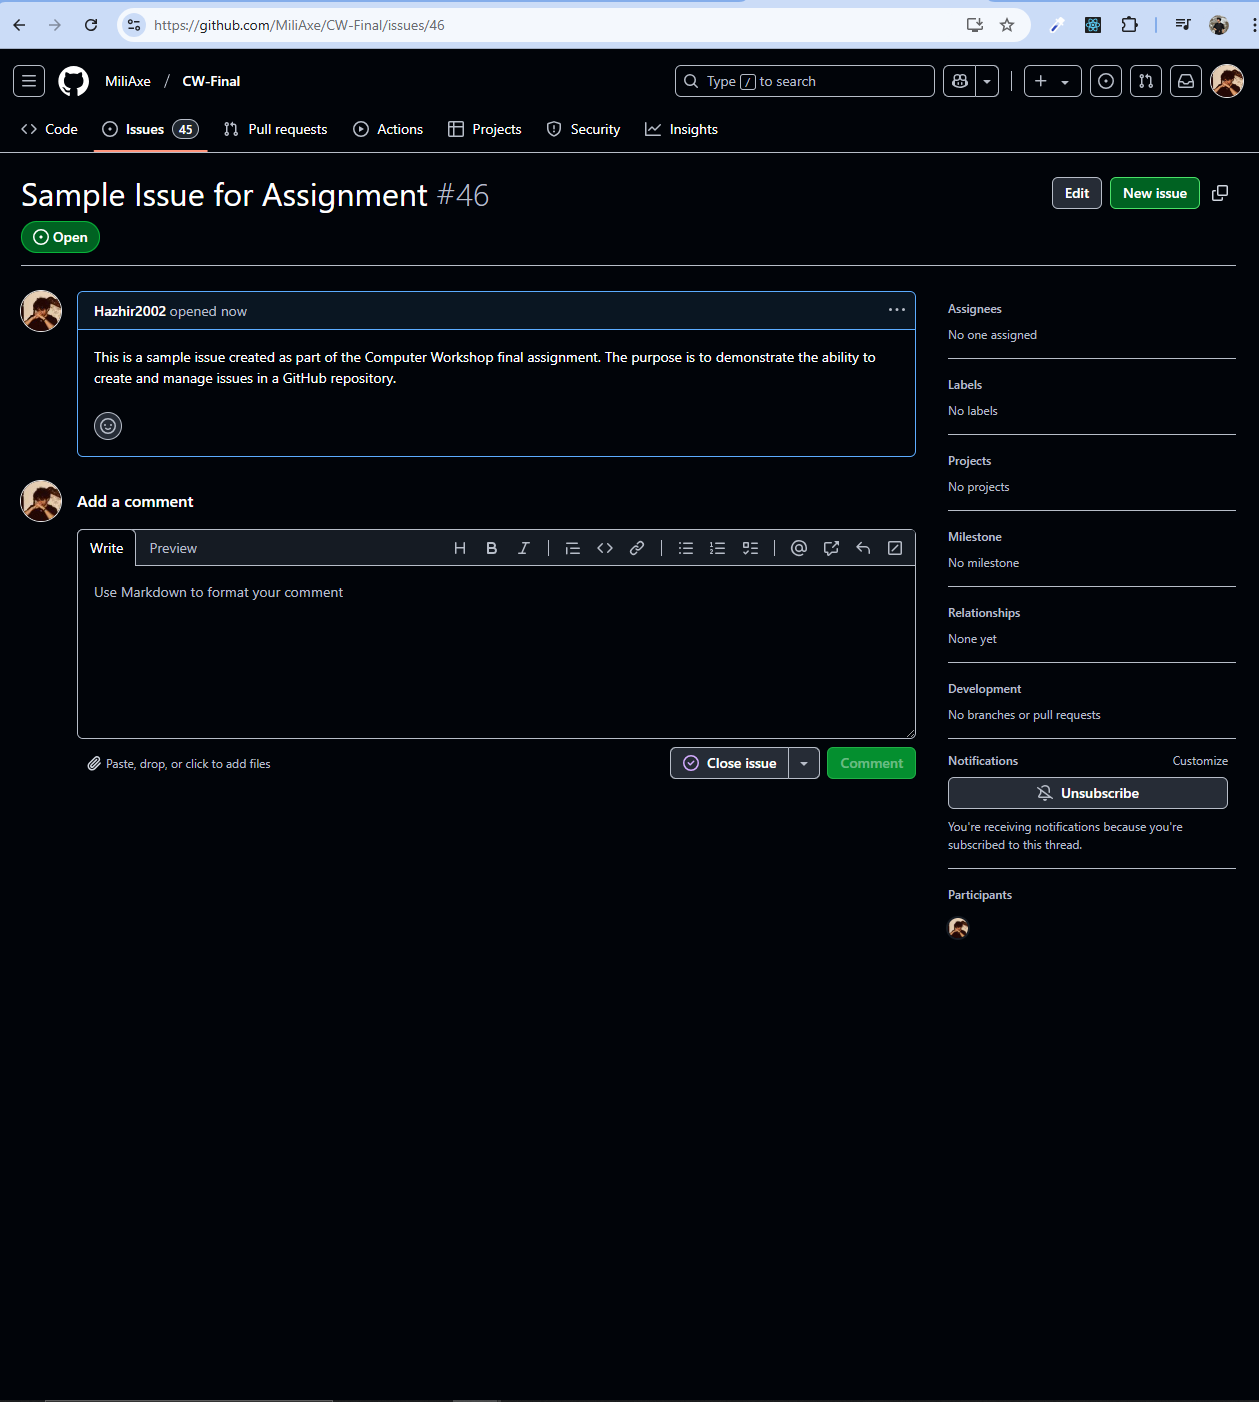
\includegraphics[width=0.8\textwidth]{issue_screenshot.png}
 \caption{Sample Issue Created in the Repository}
 \label{fig:issue}
\end{figure}

\subsection{FOSS Contribution}
Contributing to Free and Open-Source Software (FOSS) is an excellent way to collaborate with the community and enhance one's skills. 

\textbf{Do I see myself contributing to FOSS projects in the future?}  
Yes, I am highly interested in contributing to FOSS projects. Specifically, I would like to contribute to projects in the following areas:
\begin{itemize}
 \item \textbf{Web Development Frameworks:} Contributing to tools like Django or React to enhance their functionality.
 \item \textbf{Developer Tools:} Improving tools like Git or code editors (e.g., VS Code).
 \item \textbf{Educational Platforms:} Supporting open-source platforms for learning and teaching, such as Moodle or Open edX.
\end{itemize}

Contributing to FOSS is a meaningful way to give back to the developer community while learning from real-world codebases and collaborating with others.

\end{document}